The tool I implemented, called \toolname, is a \textit{Java-}program aimed at helping further developers during the testing process of their Android mobile applications. \\
For giving a cleaner and more understandable explanation how \toolname\ works, I would like to split its key features into three main categories (which should also be executed in a sequential way, in order to exploit the whole \toolname's potentiality): 
\begin{enumerate}
\item the \textsc{testing} part is in charge of testing a given set of \textit{APKs}, reporting their testing results and extracting possible \textit{crashes} from the before generated testing logs; 

\item the \textsc{clustering} part investigates the similarity between the previous extracted crash logs, using different metrics and strategies, in order to collect they together and create a crash log \textit{bucket}; 

\item the \textsc{linking} part represents the core feature of \toolname. It pre-processes a set of given \textit{user reviews} as well as the previous created set of crash logs, in order to prepare and "clean" them for the linking procedure.  Afterwards, it investigates whether it exists a correlation between the stack traces and the user feedbacks, with the aim to link, whether possible, the reviews with the crash logs. 
\end{enumerate}

\section{Testing}
%----------------- FDROID CRAWLER --------------
First of all, if there is no a set of \textit{APKs} yet, \toolname\ can be also used for downloading the needed mobile application from the \textit{F-Droid API\footnote{LINK API}}. In this direction, as shown in the picture \ref{testing}, the component \textsc{fdroid crawler}, first is in charge of  parsing a static structured file, which contains a set of android packages names. 
The path of this file is located in the \textsc{configuration manager} file, which contains a set of static properties elaborated by \toolname. Second, \textsc{fdroid crawler} searches and then extracts a set of \textit{HTTP links} for those android packages. Afterwards, it builds the correct \textit{HTTP request} in accord with the \textit{FDroid endpoint} and finally starts the downloading process, where all the found packages in the API gets downloaded and stored in a given directory. 

%-------------- SET APKS ACQUISITO --------------
Once the set of \textit{APKs} is built (either using \textsc{fdroid crawler}
or manually) and once all the parameters needed have been specified in the \textsc{configuration manager}, the testing process is able to gets started. \\
Figure \ref{config}, shows an example of parameters which must be given in order to launch the testing session. 

\label{config}
\begin{lstlisting}[caption=A set of needed parameters in order to start the testing process]
/**
* Testing logs directories
*/
MONKEY_DIR = Reports/MonkeyReports
SAPIENZ_DIR = Reports/SapienzReports

/**
 * Monkey parameters
 */
LOG_VERBOSITY = -v 
PACKAGE_ALLOWED = -p
NR_INJECTED_EVENTS = 5000
DELAY_BETWEEN_EVENTS = 10
PERCENTAGE_TOUCH_EVENTS = 15
PERCENTAGE_SYSTEM_EVENTS = 15
PERCENTAGE_MOTION_EVENTS = 15
IGNORE_CRASH = True

/**
* Sapienz parameters
*/
SEQUENCE_LENGTH_MIN = 20
SEQUENCE_LENGTH_MAX = 500
SUITE_SIZE = 5
POPULATION_SIZE = 50
OFFSPRING_SIZE = 50
GENERATION = 100
CXPB = 0.7
MUTPB = 0.3
\end{lstlisting}

In addition, the automated testing tool is going to be used has to been given as parameter in \textsc{main} \textit{args} (as mentioned in the section \ref{sec:choicetool}, either \monkey or \sapienz). 
It must be also specified on which kind of device (\textit{i.e}, a real device, such as a \textit{tablet} or a virtual device, such as an \textit{emulator}) the testing is going to be performed. 





First of all, \toolname\ recognizes all the \textit{APKs} stored in the given folder and validates its body, \textit{i.e.} whether they are able to be installed on a android mobile device.
As shown in the picture \ref{testing},  

 %and installs them one by one during the testing phase. It installs them on one or more attached mobile devices and starts the automated testing phase. It stress the AUT using the automated testing tool specified as parameter in the \textit{Main} body  







Afterwards, \toolname\ stores the from these automated testing tools generated reports, it scans them and whether a bug occurred, it extracts the \textit{crash} from the documented \textit{stack trace} and accurately writes it on a new file, in order to differentiate stack traces without crashes

\section{Clustering}

\section{Linking}

\section{How to start \toolname}
First of all, a set of parameters and directories have to inserted in the static \textit{Configuration Manager} file.


\begin{figure}[t]
\centering 
%	\vspace{-1.5mm} 
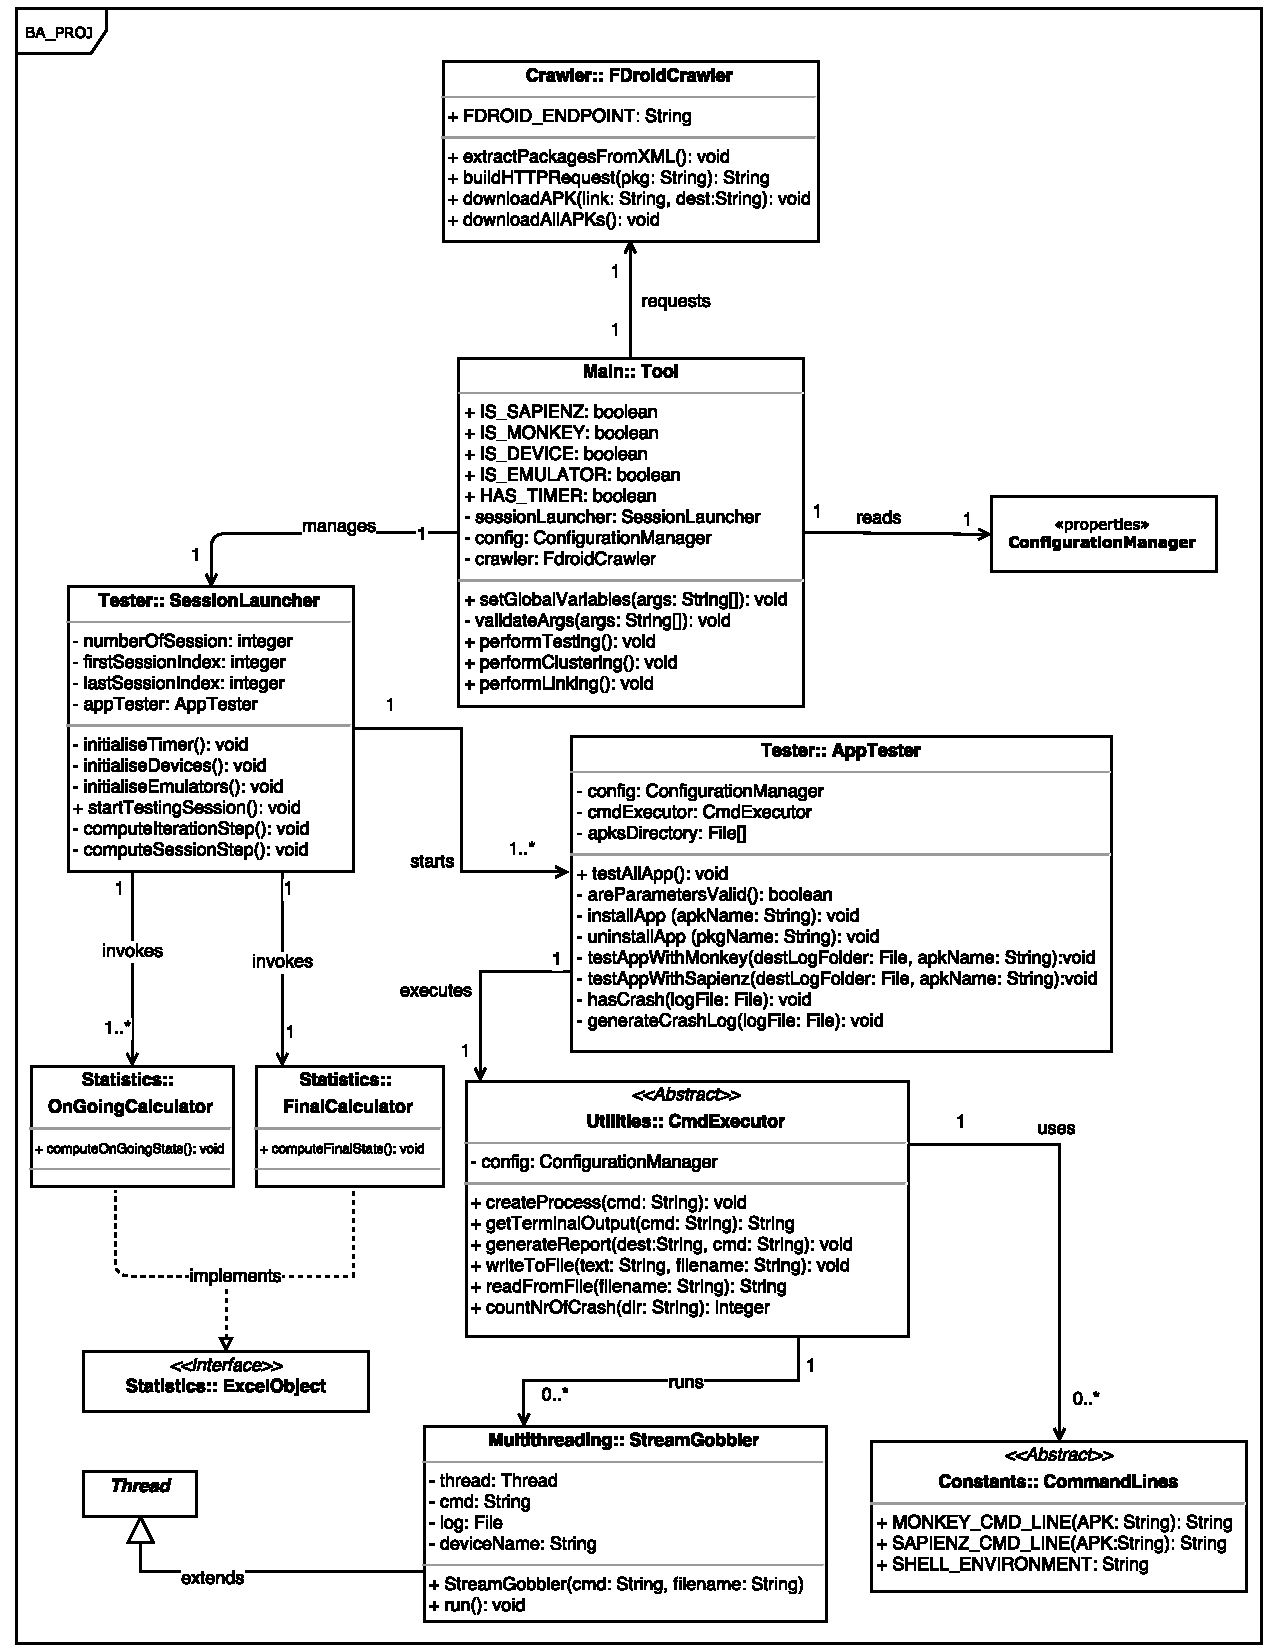
\includegraphics[width=\columnwidth]{diagrams/testing.pdf} 
\caption{Class Diagram of the testing part of the tool }
\label{testing}
\vspace{-3mm} 
\end{figure}



\begin{figure}[t]
\centering 
%	\vspace{-1.5mm} 
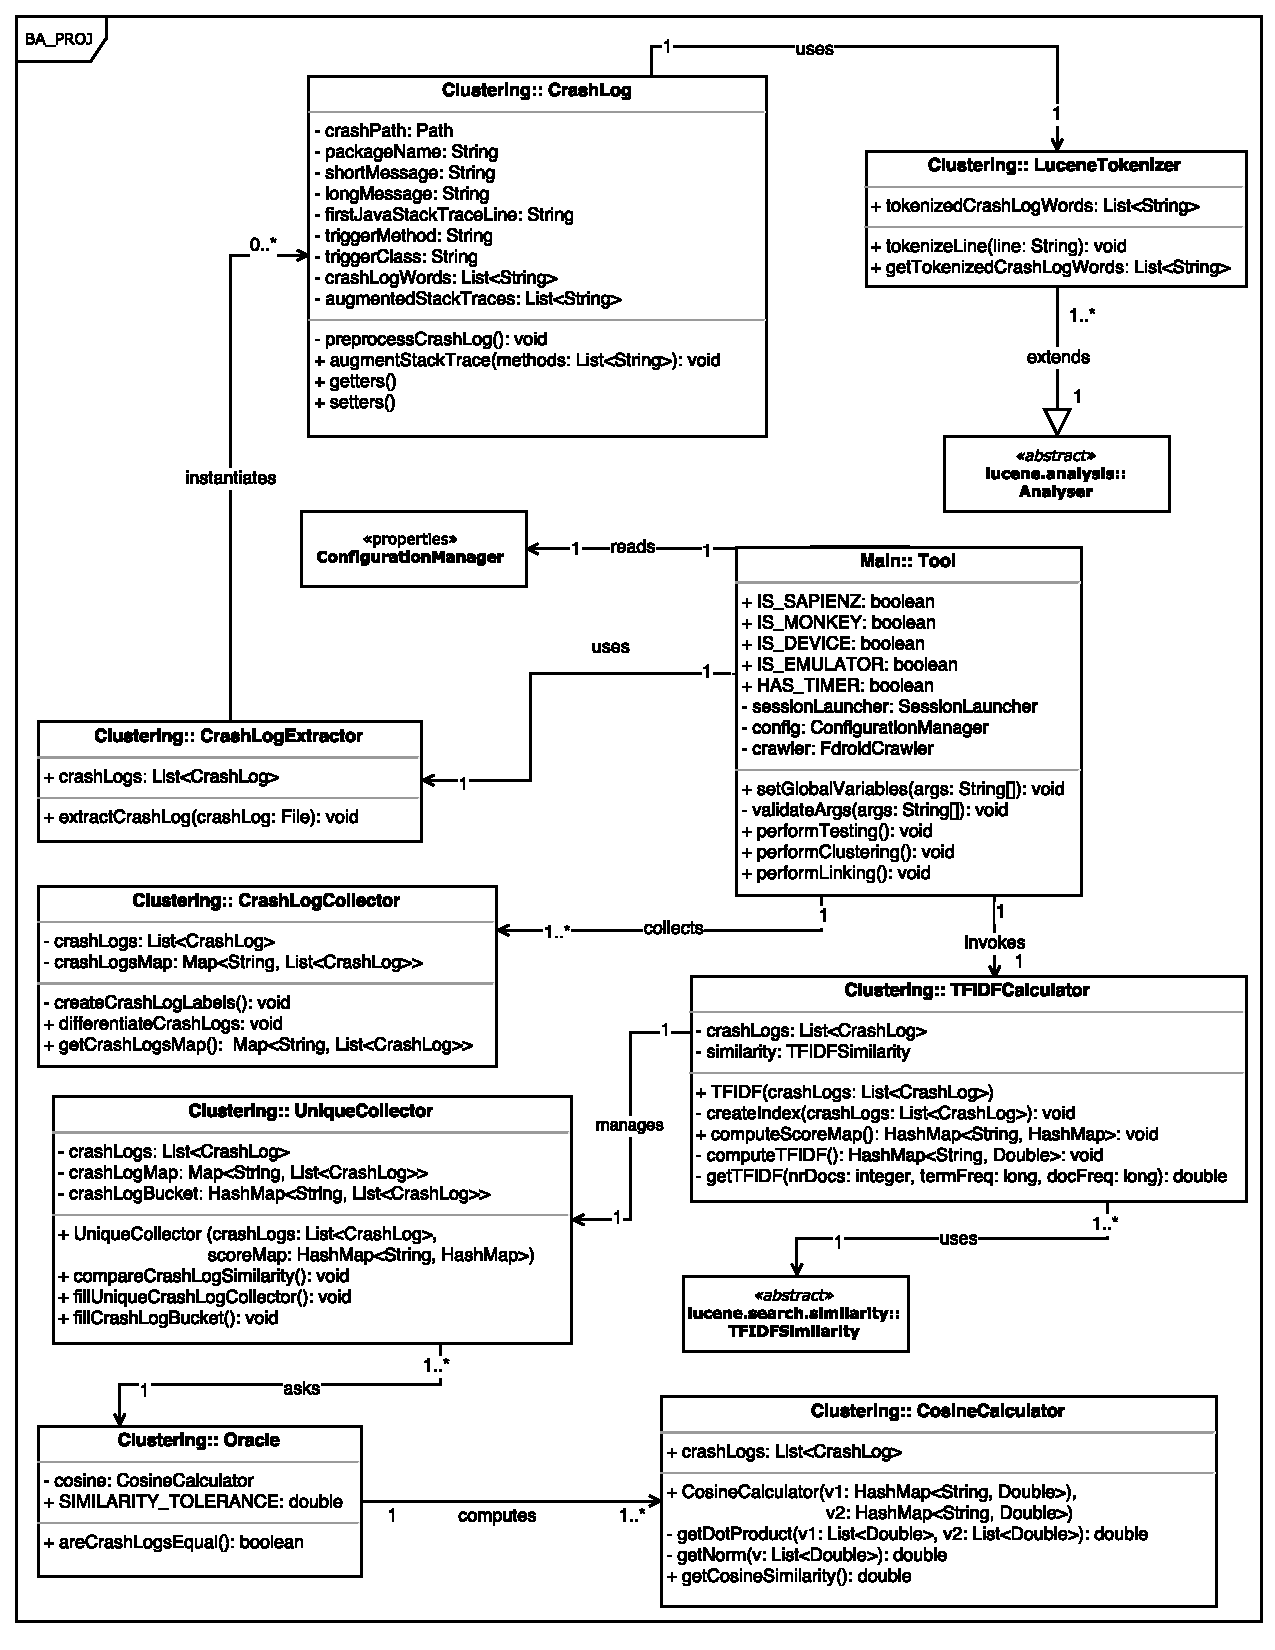
\includegraphics[width=\columnwidth]{diagrams/clustering.pdf} 
\caption{Class Diagram of the clustering part of the tool }
\label{clustering}
\vspace{-3mm} 
\end{figure}


\begin{figure}[t]
\centering 
%	\vspace{-1.5mm} 
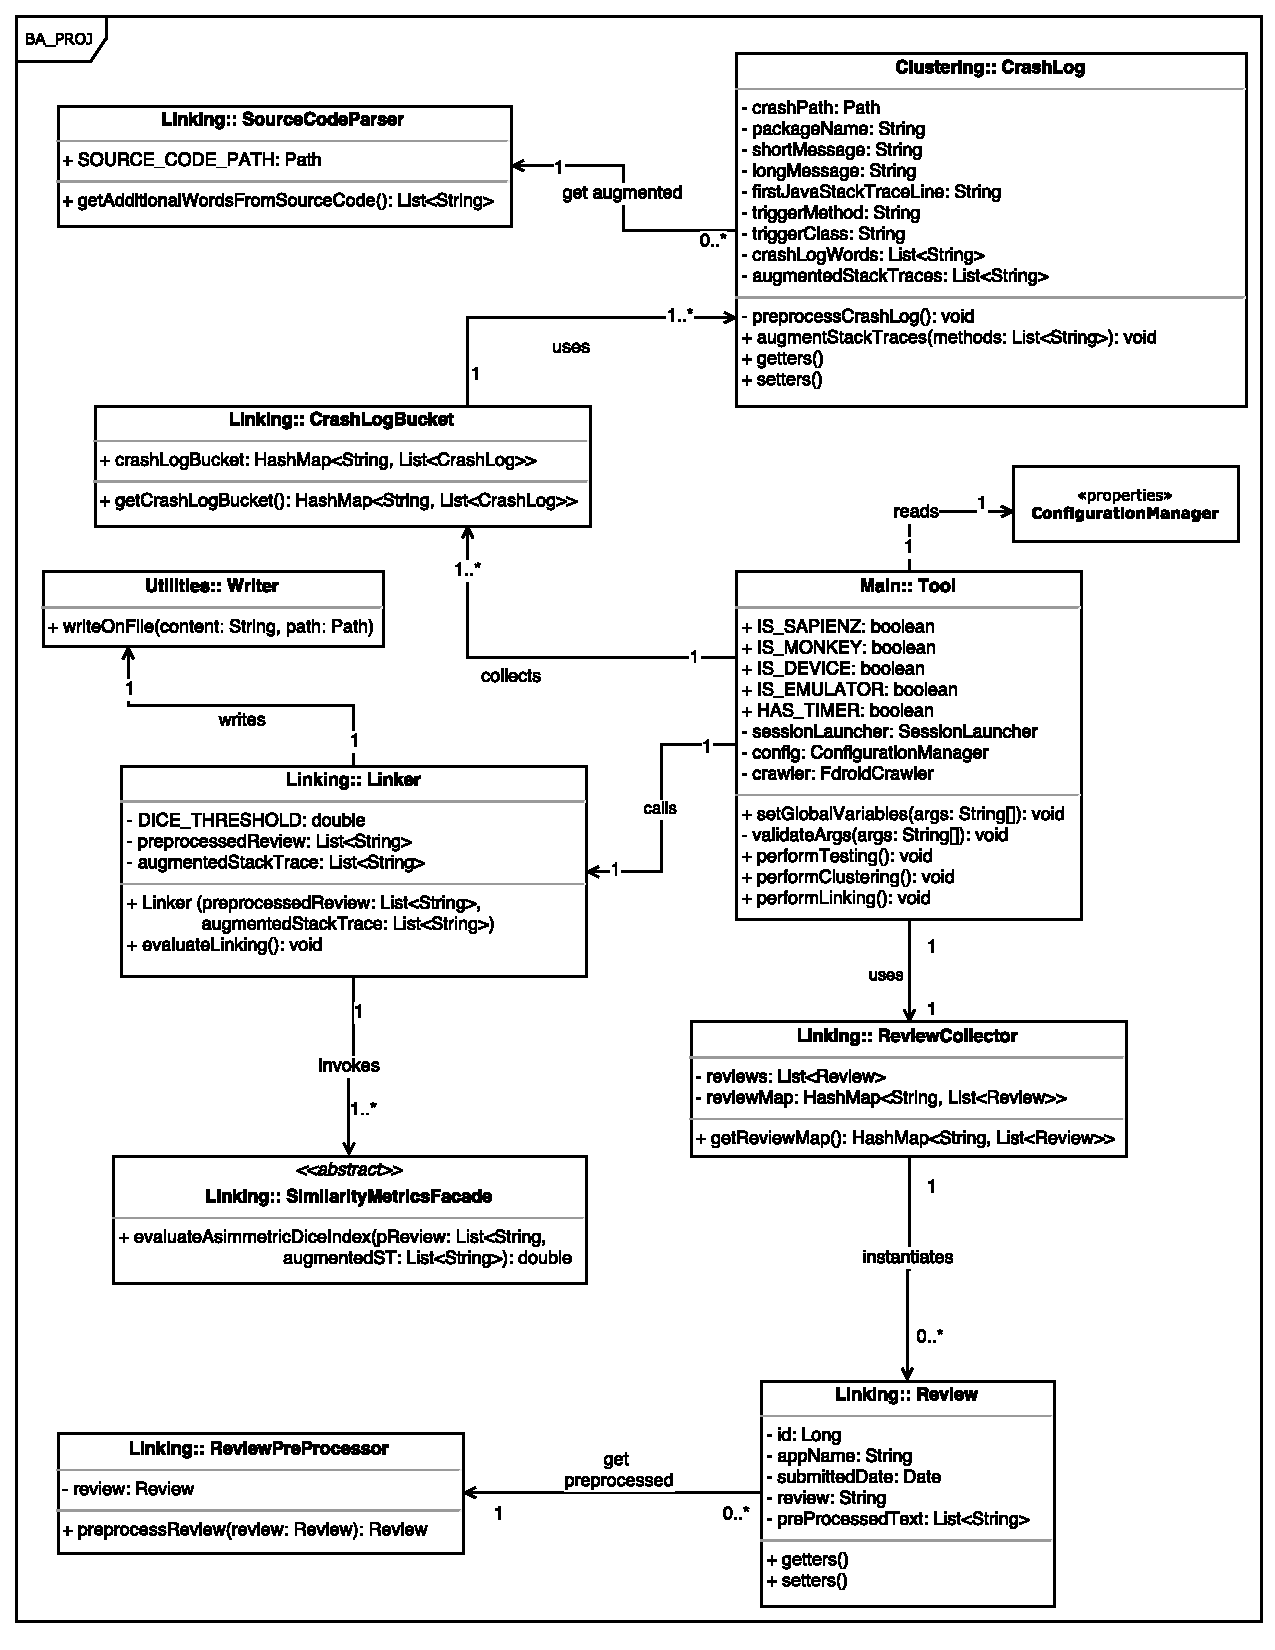
\includegraphics[width=\columnwidth]{diagrams/linking.pdf} 
\caption{Class Diagram of the linking part of the tool }
\label{linking}
\vspace{-3mm} 
\end{figure}